\documentclass[]{standalone}
\usepackage{amsmath}
\usepackage{graphicx}
\usepackage[pdf]{pstricks}
\usepackage{pgfplots}
\pgfplotsset{compat=newest}
\usepgfplotslibrary{fillbetween}
%% the following commands are needed for some matlab2tikz features
\usetikzlibrary{plotmarks}
\usetikzlibrary{arrows.meta}
\usepgfplotslibrary{patchplots}
\usetikzlibrary{decorations.text}
\usetikzlibrary{shapes.multipart}


\newcommand{\logLogSlopeTriangle}[5]
{
	% #1. Relative offset in x direction.
	% #2. Width in x direction, so xA-xB.
	% #3. Relative offset in y direction.
	% #4. Slope d(y)/d(log10(x)).
	% #5. Plot options.
	
	\pgfplotsextra
	{
		\pgfkeysgetvalue{/pgfplots/xmin}{\xmin}
		\pgfkeysgetvalue{/pgfplots/xmax}{\xmax}
		\pgfkeysgetvalue{/pgfplots/ymin}{\ymin}
		\pgfkeysgetvalue{/pgfplots/ymax}{\ymax}
		
		% Calculate auxilliary quantities, in relative sense.
		\pgfmathsetmacro{\xArel}{#1}
		\pgfmathsetmacro{\yArel}{#3}
		\pgfmathsetmacro{\xBrel}{#1-#2}
		\pgfmathsetmacro{\yBrel}{\yArel}
		\pgfmathsetmacro{\xCrel}{\xArel}
		%\pgfmathsetmacro{\yCrel}{ln(\yC/exp(\ymin))/ln(exp(\ymax)/exp(\ymin))} % REPLACE THIS EXPRESSION WITH AN EXPRESSION INDEPENDENT OF \yC TO PREVENT THE 'DIMENSION TOO LARGE' ERROR.
		
		\pgfmathsetmacro{\lnxB}{\xmin*(1-(#1-#2))+\xmax*(#1-#2)} % in [xmin,xmax].
		\pgfmathsetmacro{\lnxA}{\xmin*(1-#1)+\xmax*#1} % in [xmin,xmax].
		\pgfmathsetmacro{\lnyA}{\ymin*(1-#3)+\ymax*#3} % in [ymin,ymax].
		\pgfmathsetmacro{\lnyC}{\lnyA+#4*(\lnxA-\lnxB)}
		\pgfmathsetmacro{\yCrel}{\lnyC-\ymin)/(\ymax-\ymin)} % THE IMPROVED EXPRESSION WITHOUT 'DIMENSION TOO LARGE' ERROR.
		
		% Define coordinates for \draw. MIND THE 'rel axis cs' as opposed to the 'axis cs'.
		\coordinate (A) at (rel axis cs:\xArel,\yArel);
		\coordinate (B) at (rel axis cs:\xBrel,\yBrel);
		\coordinate (C) at (rel axis cs:\xCrel,\yCrel);
		
		% Draw slope triangle.
		\draw[#5]   (A)-- node[pos=0.5,anchor=north] {1}
		(B)-- 
		(C)-- node[pos=0.5,anchor=west] {#4}
		cycle;
	}
}
\begin{document}
	
	
	
	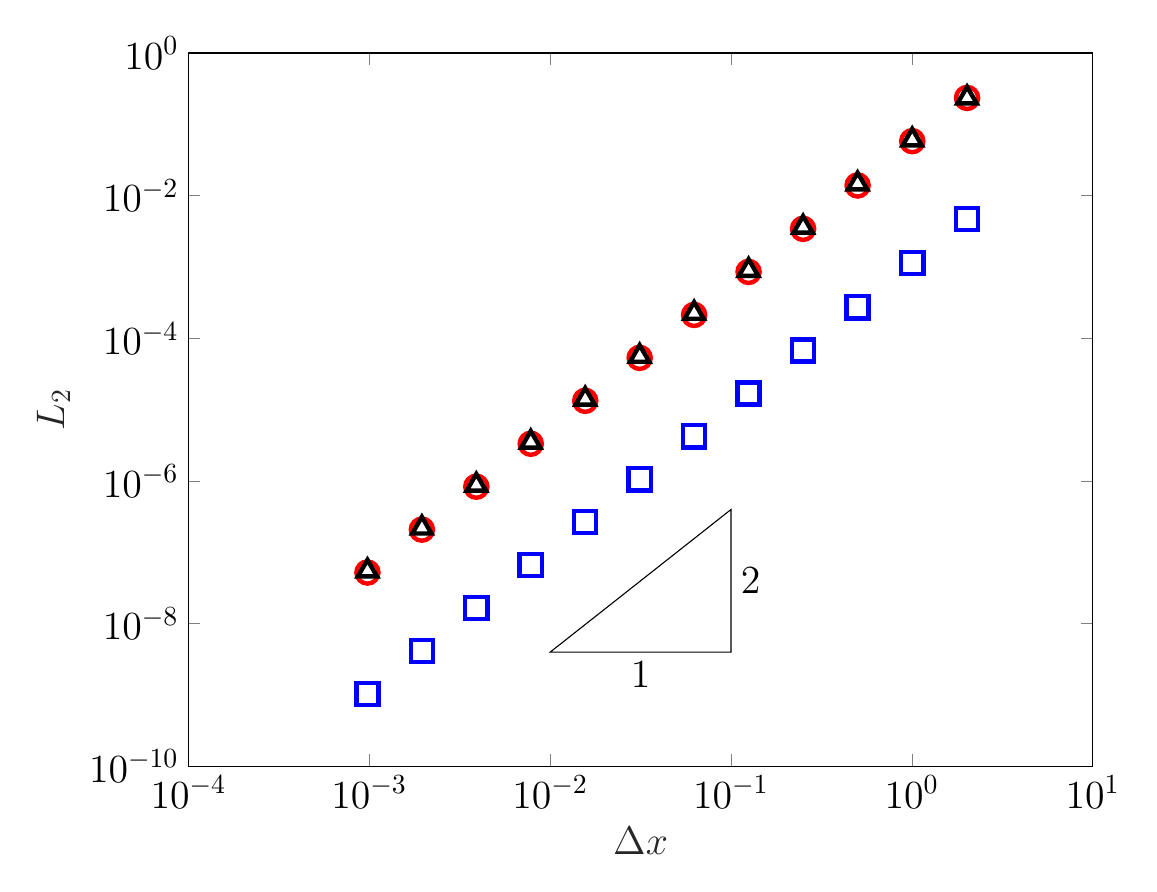
\begin{tikzpicture}
	\tikzstyle{every node}=[font=\Large]

\begin{axis}[%
width=4.521in,
height=3.566in,
at={(0.758in,0.481in)},
every axis plot/.append style={ultra thick},
scale only axis,
xmode=log,
xmin=0.0001,
xmax=10,
xtick={0.0001,  0.001,   0.01,    0.1,      1,     10},
xminorticks=false,
xlabel style={font=\color{white!15!black}},
xlabel={\Large $\Delta x$},
ymode=log,
ymin=1e-10,
ymax=1,
ytick={ 1e-10,  1e-08,  1e-06, 0.0001,   0.01,      1,    100},
yminorticks=false,
ylabel style={font=\color{white!15!black}},
ylabel={\Large $L_2$},
axis background/.style={fill=white}
]

 \logLogSlopeTriangle{0.6}{0.2}{0.16}{2}{black};
 
\addplot [color=blue, draw=none, mark=square, mark size=4pt, mark options={solid, blue}, forget plot]
  table[row sep=crcr]{%
2.02020202020202	0.00469476869927846\\
1.00502512562814	0.00113059903015153\\
0.50125313283208	0.000272823148753446\\
0.250312891113892	6.76245750555735e-05\\
0.125078173858662	1.6892023560867e-05\\
0.0625195373554236	4.22561764345097e-06\\
0.0312548835755587	1.05701901218963e-06\\
0.0156262207984999	2.64354463273367e-07\\
0.00781280518770264	6.61022583618534e-08\\
0.00390632629543546	1.65272571703105e-08\\
0.00195314407367259	4.13162677494295e-09\\
0.000976567268394865	1.03292223001934e-09\\
};
\addplot [color=red, draw=none, mark=o, mark size=4pt, mark options={solid, red}, forget plot]
  table[row sep=crcr]{%
2.02020202020202	0.234717674690414\\
1.00502512562814	0.0581336463603201\\
0.50125313283208	0.0139128252532896\\
0.250312891113892	0.00342898030531673\\
0.125078173858662	0.000853273117625569\\
0.0625195373554236	0.000212978223209787\\
0.0312548835755587	5.32120676225566e-05\\
0.0156262207984999	1.32998495114909e-05\\
0.00781280518770264	3.3246024948889e-06\\
0.00390632629543546	8.31097791699236e-07\\
0.00195314407367259	2.07772407722966e-07\\
0.000976567268394865	5.19811263189575e-08\\
};
\addplot [color=black, draw=none, mark=triangle, mark size=4pt, mark options={solid, black}, forget plot]
  table[row sep=crcr]{%
2.02020202020202	0.235188799159603\\
1.00502512562814	0.0605165167407834\\
0.50125313283208	0.0146681030936224\\
0.250312891113892	0.00361900289807826\\
0.125078173858662	0.000900549628840602\\
0.0625195373554236	0.000224762155999577\\
0.0312548835755587	5.61536542374343e-05\\
0.0156262207984999	1.40347329547496e-05\\
0.00781280518770264	3.50825941605018e-06\\
0.00390632629543546	8.77002872394135e-07\\
0.00195314407367259	2.19249670961135e-07\\
0.000976567268394865	5.48052729511495e-08\\
};
\end{axis}
\end{tikzpicture}%
\end{document}